\section*{Proving the correctness of the mystery function%
\TAGS{correctness}}

We use contracts to both test our code and to reason about code. With
contracts, careful point-to reasoning and good testing both help us to
be confident that our code is correct.

Here's a different way of looking at the mystery function from lecture.
Once we have loop invariants for the mystery function, we can view the
whole thing as a control flow diagram:
\begin{center}
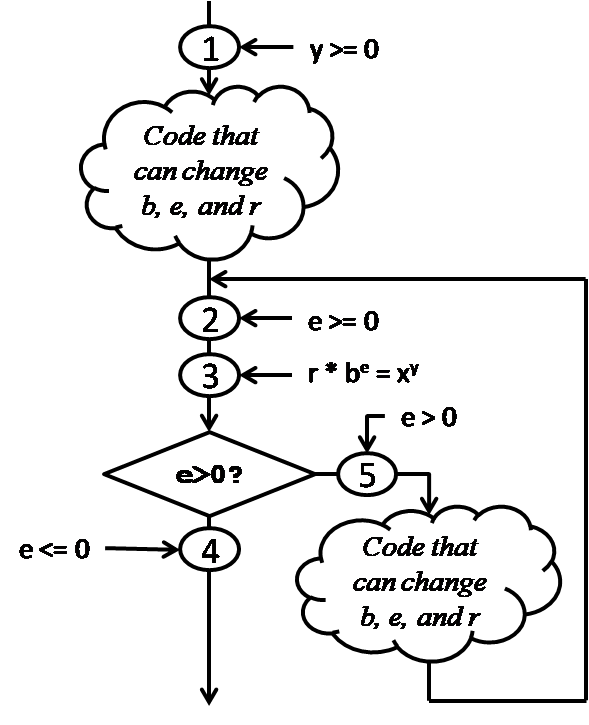
\includegraphics[width=0.4\textwidth]{\img/fastpow-control-flow.png}
\end{center}
\begin{sloppypar}
The circle labeled \textbf{1} is a \shortanswerline{precondition} of
the function, and the circles labeled \textbf{2} and \textbf{3} are
\shortanswerline{loop invariants}. The circles labeled \textbf{4} and
\textbf{5} just capture information we get from the result of the loop
guard (or loop condition), but we might write \textbf{4} as an
\shortanswerline{$\backslash$assert} statement.
\end{sloppypar}

\enlargethispage{5ex}
To prove this function correct, we need to reason about the two pieces
of code (pieces that this diagram hides in the two cloud-bubbles) to
ensure that our contracts never fail:
\begin{itemize}
  \item When we reason about the upper code bubble, we assume that
    \shortanswerline{~~\textbf{1}~~} is true before the code runs and show that
    \shortanswerline{~~\textbf{2}~~} and
    \shortanswerline{~~\textbf{3}~~} are true afterwards.  (This is INITialization.)
  \item When we reason about the lower code bubble, we assume
    \shortanswerline{~~\textbf{2}~~}, \shortanswerline{~~\textbf{3}~~}, and
    \shortanswerline{~~\textbf{5}~~} are true before the
    code runs and show that \shortanswerline{~~\textbf{2}~~} and
    \shortanswerline{~~\textbf{3}~~} are true
    afterwards.  (This is PREServation.)
  \item To reason that the returned value $r$ is equal to $x^y$, we
    combine the information from circles \shortanswerline{~~\textbf{2}~~} and
      \shortanswerline{~~\textbf{4}~~} to conclude that $e = 0$.  Together with
    the information in circle
    \shortanswerline{~~\textbf{3}~~}, this implies that $r = x^y$.
    (This is correctness on EXIT.)
\end{itemize}

In addition, we have to reason about TERMination: every time the lower
code bubble runs, the value $e$ gets strictly smaller, because $e/2 <
e$ for every $e > 0$, and the loop invariant ensures $e$ never becomes
negative.

\clearpage
To summarize, in general there are four steps for proving the
correctness of a function with one loop using loop invariants:
\begin{itemize}
\item%
  \answerline{Showing that the loop invariant is true INITially}
\item%
  \answerline{Showing that the loop invariant is PREServed by any iteration}
\item%
  \answerline{Showing that the loop invariant and negation of the loop
    guard implies postcondition on EXIT}
\item%
  \answerline{Showing that the loop always TERMinates}
\end{itemize}
